% TEMPLATE for Usenix papers, specifically to meet requirements of
%  USENIX '05
% originally a template for producing IEEE-format articles using LaTeX.
%   written by Matthew Ward, CS Department, Worcester Polytechnic Institute.
% adapted by David Beazley for his excellent SWIG paper in Proceedings,
%   Tcl 96
% turned into a smartass generic template by De Clarke, with thanks to
%   both the above pioneers
% use at your own risk.  Complaints to /dev/null.
% make it two column with no page numbering, default is 10 point

% Munged by Fred Douglis <douglis@research.att.com> 10/97 to separate
% the .sty file from the LaTeX source template, so that people can
% more easily include the .sty file into an existing document.  Also
% changed to more closely follow the style guidelines as represented
% by the Word sample file. 
% This version uses the latex2e styles, not the very ancient 2.09 stuff.
\documentclass[twocolumn, 10pt]{article} 
\setlength{\columnsep}{0.15in}
\usepackage{graphicx,fullpage,epsf,epsfig,endnotes}
\usepackage[T1]{fontenc}
\usepackage{pslatex}
\usepackage{times}
\begin{document}

%make title bold and 14 pt font (Latex default is non-bold, 16 pt)
\title{\Large \bf Capture, conversion, storage, and analysis of an intense NFS workload}

\author{
\begin{tabular}{c}
Eric Anderson
eric.anderson4@hp.com \\
\end{tabular}
}

\maketitle

% Use the following at camera-ready time to suppress page numbers.
% Comment it out when you first submit the paper for review.
%\thispagestyle{empty}

\subsection*{Abstract}
We describe methods to capture, convert, store and analyze NFS
workloads that are 20-100$\times$ more intense, in terms of
operations/day, than any previously published.
%
We describe three techniques that improve capture performance by up to
$10\times$ over previous techniques.
%
For conversion, we use a general-purpose format that is both highly
space efficient and provides efficient access to the trace data.
%
For
analysis, we describe a number of techniques adopted from the
database community and some new techniques that facilitate analysis of 
very large traces.
%
We also describe a number of guidelines for trace collection that should
prove useful to future practitioners.
%
Finally, we analyze a commercial feature
animation (movie) rendering workload using these techniques and discuss the
characteristics of the workload.
%
Our implementation of these techniques is available as open source
and the exact anonymized datasets we analyze are available for free download.

% LocalWords:  anonymized


\section{Introduction}

\fix{11. Another word rather than intense in title?}
\fix{13. More motivation on why we do tracing -- if we can get the space}
Storage tracing and analysis has a long history.  Some of the earliest
filesystem traces were captured in 1985~\cite{ousterhout85}, and there
has been intermittent tracing effort since then, summarized by
Leung~\cite{LeungUsenix08}.  These traces are
analyzed to find properties that future systems should support or
exploit, and as input to simulators and replay tools to explore system
performance with real workloads.

One of the problems
with trace analysis is that old traces inherently have to be scaled up
to be used for evaluating newer storage systems because the
underlying performance of the newer systems has increased.  Therefore,
the community benefits from regularly capturing new traces from multiple
sources, and if possible, traces that put a heavy load on the storage
system, reducing the need to scale the workload.

Most traces, since they are performed by academics, are captured in
academic settings.  This means that the workloads captured are
somewhat comparable, but it also means that commercial workloads are
under-emphasized.  Microsoft is working to correct this by capturing
commercial enterprise traces from their internal
servers~\cite{snia-iotta-microsoft}.  Our work focuses on commercial
NFS~\cite{rfc1094nfs} workloads, in particular from a feature animation (movie) company.
The name of the company remains blinded as part of the agreement to
publish the traces.  The last publically available NFS traces that we
are aware of were collected in 2003.  Our 2003 and 2007
traces~\cite{animation-bear-traces} provide recent NFS traces for use
by the community.

One difference between our traces and other ones is the data rates
that we measured.  Our 2003 client traces saw about 750 million
operations per day.  In comparison, the 2003 Ellard
traces~\cite{EllardLisa03} saw a peak of about 125 million NFS
operations per day, and the 2007 Leung traces~\cite{LeungUsenix08}
saw a peak of 19 million CIFS operations/day.  Our 2007 traces saw
about 2.4 billion operations/day.  This difference required us to
develop and adopt new techniques to capture, convert, and analyze the
traces.

Since our traces were captured in such a different environment than
prior traces, we limit our comparisons to their workloads, and we
do not attempt to make any claims about trends.  We believe that
unless we, as a community, collect traces from hundreds of different
sites, we will not have sufficient data to make claims stronger than
``this workload is different from other ones in these ways.''  In
fact, we make limited comparison in the trends between our 2003 and
2007 traces for similar reasons.  The underlying workload changed
as the rendering techniques improved to generate higher quality output,
the operating system generating the requests changed, the NFS
protocol version changed, and the configuration of the clients 
changed because of standard technology trends.

The process of understanding a workload involves four main
steps, as shown in Figure~\ref{fig:overall-process}.  Our tools for
these steps are shown in italics for each step, as well as some
traditional tools.  The first step is capturing the workload, usually
as some type of trace.  The second step is conversion, ususally from
some raw format into a format designed for analysis.  The third step
is analysis to reduce the huge amount of converted data to
something manageable.  Alternately, this step is a simulation or replay to
explore some new system architecture.  Finally the fourth step is to
generate graphs or textual reports from the output of the analysis or
simulation.

Our work has five main contributions:

\begin{enumerate}
\item The development of techniques for lossless raw packet capture up to
5Gb/s, and with the hardware improvements since our work, likely to
10Gb/s.  These techniques are applicable to anyone wanting to capture
a network storage service such as NFS, CIFS, or iSCSI.

\item A series of guidelines for the conversion and storage of the
traces.  Many of these guidelines are things that we wish we had known
when we were converting our traces.  We used
DataSeries~\cite{DataSeriesOSR2009} to store the traces, but our
guidelines are general.

\item Improved techniques for analyzing very large traces that allow
us to look at the burstiness in workloads, and an examination of how
the long averaging intervals in prior analysis can obscure workload
properties.

\item The analysis of an intense NFS workload demonstrating that our
techniques are successful.

\item The agreement with the animation company to allow the roughly
100 billion operation anonymized traces to be published, along with
the complete set of tools to perform all the analysis presented in
this paper and to generate the graphs.  Other
researchers can build on our tools for further analysis, and use
the traces in simulation studies.
\end{enumerate}

\begin{figure}
\center 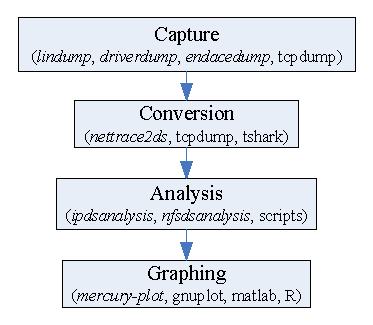
\epsfig{width=2.2in, angle=0, file=overall-process.eps}
\caption{Overall process; our tools are shown in italics, traditional tools
after them.}
\label{fig:overall-process}
\end{figure}

We examine related work in section~\ref{sec:related}.  We describe our
capture techniques in section~\ref{sec:capture}, followed by the
conversion (section~\ref{sec:conversion}). We describe our adopted and
new analysis techniques in section~\ref{sec:analysis-techniques} and
use them to analyze the workload in section~\ref{sec:analysis}.
Finally we conclude in section~\ref{sec:conclusion}.

\section{Capture}
\label{sec:capture}

The first stage in analyzing an NFS workload is capturing the data.
There are three places that the workload could be captured: the
client, the server, or the network.  Capturing the workload on the
clients is very parallel, but is difficult to configure and can
interfere with the actual workload.  Capturing the workload on the
server is straightforward if the server supports capture, 
but impacts the performance of the
server.  Capturing the workload on the network through port mirroring
is about as convenient as capture on the server, and given that most
switches implement mirroring in hardware, has no impact on network or
workload performance.  On fiber networks, even the potential impact of
port mirroring can be eliminated through the use of optical fiber
splitters. Therefore, we have always chosen to capture the
data through the use of port mirroring.

A single mirror port could be insufficient for mirroring both the send
and recieve directions of a full-duplex port.  However, advanced
switches can selectively mirror each direction of a port onto
particular ports.  We used this functionality in our 2003 tracing to
spread 2-4 one Gbit links over 2 one Gbit mirror ports.

Even if 1 second average rates are low enough to fit onto the mirror
ports, if the switch has insufficient buffering, packets can still be
dropped. We discovered this problem on a switch that used per-port
rather than per-card buffering.  To eliminate the problem, we switched
to 10Gbit mirror ports to reduce the need for switch-side buffering.

The capture host can also be overrun. At low data rates (900Mbits,
70kpps), standard tcpdump on commodity hardware works fine.
However, at high data rates (5000Mbits, 1,000kpps),
traditional approaches are insufficient. Indeed,
Leung\cite{LeungUsenix08} notes
% pg 215 ``when tcpdump dropped a few packets''
difficulties with packet loss using tcpdump on a 1 Gbit mirror port.
We have developed three separate techniques for packet capture, all of
which work better than tcpdump: {\it lindump}(user-kernel ring
buffer), {\it driverdump}(in-kernel capture to files), and {\it
endacedump}(hardware capture to memory).  Further details and
experiments with the first two techniques can be found
in~\cite{Anderson06network-tracing}.

\subsection{Lindump}

The linux kernel includes a memory-mapped, shared ring buffer for
packet capture.  We modified the example lindump program to write out
pcap files~\cite{pcap}, the standard output format from tcpdump, and
to be able to capture from more than one interface at the same time.
We wrote the output files to an in-memory filesystem using mmap to
reduce copies, and copied and compressed the files in parallel to
disk.  Using an HP DL580G2, a current 4 socket server circa 2003,
lindump was able to capture about 3x the packets per second (pps) as
tcpdump and about 1.25x the bandwidth.  Combined with a somewhat
higher burst rate while the kernel and network card buffered data,
this was sufficient for mostly loss free captures at the animation
company, and was the technique we used for all of the 2003 set of
traces.

Once our packets are captured into files in tmpfs, we used compression
to maximize the effective disk space.  If the capture host is mostly
idle, we compressed with {\tt gzip -9}. As the backlog of pending
files increased, we reduced the compression algorithm to {\tt gzip
-6}, then to {\tt gzip -1}, and finally to nothing.  In practice this
approach increased the effective disk size by 1.5-2.5x in our
experience as the data was somewhat compressible, but at higher input
rates we had to fall back to reduced compression.

\subsection{Driverdump}

At a second site, our 1Gbit lindump approach was insufficient because
of packet bursts and limited buffering on the switch.  Replacing the
dual 1Gbit cards with a 10GbE card merely moved the bottleneck to the
host and the packets were dropped on the card before they could be
consumed by the kernel.

To fix this problem, we modified the network driver so that instead of
passing packets up the network stack, it would just copy the packets
in pcap format to a file. Then it would immediately return the packet
buffer to the NIC.  A user space program prepared files for capture,
and closed the files on completion.  We called our solution {\tt
driverdump} since it performed all of the packet dumping in the
driver.

Because driverdump avoids the kernel IP stack, it could
capture packets faster than the IP stack could drop them.
% measured by using tcpdump with a filter that drops all packets. 
We increased the sustained packets per second over lindump by 2.25x to
676,000pps, and sustained bandwidth by 1.5x to 170MiB/s.  We could
handle short bursts up to 900,000 pps, and 215 MiB/s.  This gave us
nearly lossless capture to memory at the second site.  Since the files
were written into tmpfs, we re-used our technology for compressing and
copying the files out to disk.

\subsection{Endacedump}

In 2007, we returned to the animation company to collect new traces on
their faster NFS servers and 10GbE network.  While an update of
driverdump might have been sufficient, we decided to also try the
Endace DAG 8.2X capture card~\cite{endace-cards}.  This card copies
and timestamps packets from a 10GbE network directly into memory.  As
a result, it can capture minimal size packets at full bandwidth, and
is intended for doing in-memory analysis of networks.  Our challenge
was to get the capture out to disk, which was not believed to be
feasable by our technical contacts at Endace.

To solve this problem, we integrated our adaptive compression
technique into a specialized capture program, and added the
lzf~\cite{lzf} compression algorithm, that compresses at about
100MB/s.  We also upgraded our hardware to an HP DL585g2 with 4 dual
core 2.8GhZ Opterons, and 6 14 disk SCSI trays.  Our compression
techniques turned our 20TiB of disk space into 30TiB of effective disk
space.  We experienced a very small number of packet drops because our
capture card limited a single stream to PCI-X bandwidth (8Gbps), and
required partitioning into two streams to capture 10GbE.  Newer cards
capture 10GbE in a single stream.

\subsection{Discussion}

Our capture techniques are directly applicable to anyone attempting to
capture data from a networked storage service such as NFS, CIFS, or
iSCSI.  Our most advanced techniques are capable of lossless
full-packet capture at 10GbE, but require the use of special hardware.
Our simplest technique allows capture at over twice the rate of
tcpdump, and expands the effective size of the disks by 1.5x through
adaptive compression. Our intermediate technique increases the capture
rates by a factor of 2-3x at the cost of development time.  Both the
lindump and driverdump code are available in our source
distribution~\cite{DSOpenSource}.  These tools and techniques should
eliminate problems of packet drops for capturing storage traces.

\section{Conversion}
\label{sec:conversion}

Once the data is captured, the second problem is parsing and
converting that data to a usable format.  There are three main
challenges in conversion: representation, performance and obfuscation.
Representation is the challenge of deciding the logical structure of
the converted data.  Performance is the challenge of making the
conversion run quickly, hopefully faster than the capture stage.
Obfuscation is the challenge of hiding important information present
in the data and is necessary for being able to release traces.


\subsection{Representation}

One option for the representation is the format used in the
Ellard\cite{ellardTraces} traces: one line per request or reply in the
file with field names to identify the different parameters in the RPC.
However, this format works poorly for representing things like
readdir, which have an arbitrary number of response fields, and though
we didn't initially implement readdir, we knew that we would want to
in the future, and since we now have, the ability to associate
multiple response parts with a single response is important.
Therefore, we chose to use a more relational data
structuring~\cite{codd70relational}.  We have a primary data table
with the common fields present in every request or reply, and an
identifier for each rpc.  We then have secondary tables that contain
request-type specific information, such as a single table for RPC's
that include attributes, and a single table for read and write
information.  We then join the common table to the other tables when
we want to perform an analysis that uses information in both.

The relational structuring improves flexibility, and allows for
analysis that only need a subset of the data to avoid reading
unnecessary parts.  For example an analysis only looking at operation
latency can simply scan the common table.

\subsection{Performance}

In order to perform the conversion in parallel, we need to divide all
of the collected files into groups and process them in parallel.
Since we need to assign each request or reply a unique id, we actually
make two passes through the data.  First we parse the data and count
the number of requests or replies, we then use those counts to
determine the first number for each group, and hence we can process
the data in parallel.  Since NFS parsing requires the request to parse
the reply, we currently do not parse any request-reply pairs that
cross a group boundary.  Similarly, we do not do full TCP
reconstruction, so for NFS over TCP, we can fail to parse requests or
replies that are not aligned with the start of a packet.  We will
parse multiple request or replies in a single packet.  These
limitations are similar to earlier work, so we found them acceptable.
The 8x speedup we get by converting in parallel means that we can
complete the conversion of a full data set (30TiB) in about 3 days.

We also chose to convert from disk files rather than try to convert
data on the fly.  We did this for simplicity, but it had the side
benefit that we could write our converter to be paranoid and
conservative, rather than have it try to recover from conversion
problems.  This helped greatly when we were handling new trace files
with new failure modes in the underlying data, and has helped reduce
the number of glitches in our converted data.  The next time we
convert data, we plan to extend our conversion tools to work
incrementally, such that we can process the first set of files while
the capture is still running, delete those files, and therefore
capture a theoretically unbounded length of trace.  We briefly
considered parallelizing the conversion across multiple machines, but
when we examined the conversion rate we were getting on our 8 core
machine, we realized that the 1Gbit network connection the tracing
machine had would be the bottleneck and would result in slower
conversion.

\subsection{Obfuscation}

In order to release the traces, we have to obscure private data such
as filenames.  There are three primary ways to perform the obfuscation: 

\begin{enumerate}

\item {\bf map values to unique integers}.  This option results in the
most compact identifiers.  It presents difficulties in parallelizing
the conversion since all identical values need to map to identical
integers.  To maintain consistent mappings between capture sessions,
the translation table needs to be maintained, which means that the
size of that table could get very large.  Finally, converting back to
the original data means that the translation table needs to be preserved.

\item {\bf map values to hash/hmac}.  This option results in larger
identifiers since secure hash's are 16-20 bytes in length.  It
eliminates the problem with parallelizing the conversion since the
hash can be calculated in parallel.  If a simple hash is used, then
this conversion is open to a dictionary attack, which may or may not
matter.  The main disadvantage of this approach is that converting
back to the original data requires that a translation table of hmac ->
original string needs to be preserved.  There is a potential problem
of collisions, but this is sufficiently implausible as to be an
ignorable problem.

\item {\bf map values to encrypted values}.  This option results in
the longest identifiers since the encrypted value will be at least as
large as the original value.  It is as parallelizable as the hash/hmac
approach, it is not open to a dictionary attack, and it can be
reversed provided the key files are kept around.

\end{enumerate}

We chose the last approach because we wanted to be able to have
discussions with the customer about results of analysis, and we needed
to be able to tell them the actual pathnames involved in what we
found.  Our encryption process embeds a prefix of the hash in the
decrypted data so that we can verify that a particular string should
be decrypted.  This allows us to write a decryption filter that looks
for hexadecimal strings in output, attempts to decrypt them, and if
successful substitutes in the decrypted data.  We have used the
reversible decryption to verify analysis of the data.  For example, a
colleague analyzed the directory structure, and wanted to identify the
strings representing '.' and '..'.  We verified through decryption
that they had identified the correct strings.

A second question is what if any parsing should be done of values
before they are encrypted.  For example, should a filename and suffix
be encrypted separately.  This question depends on what analysis will
be run in the future.  In our case, we chose to encrypt entire
filenames since the suffixes are specific to the animation process and
are unlikely to be useful to people.  This was also the most
conservative position; we could (through decryption) change our
position on this in the future.

Since most of the other values in our traces were semi-random (IP
addresses in the 10.* network, filehandles selected by the filers), we
chose to pass those values through unchanged.  If there were public
values in the traces, then we would have had to apply more
sophisticated anonymization~\cite{ruoming07anonymization}.




\section{Storage}
\label{sec:storage}

Having decided to use a relational structuring for our data, we next
needed to decide how to store the data.  There were three primary
options available to us: text, SQL, and our custom binary
format~\cite{DSTechnicalReportSnapshot} for storing trace data.  Text
is a traditional way of storing trace data, however, we were concerned
that a text representation would be too large and too slow.  Having
later converted the Ellard traces to our format, we found that the
analysis distributed with the traces used 25x less CPU time .  This
disparity convinced us that text is an inappropriate format for
storage of our traces.

% cat .../*-log | perl .../DataSeries/doc/fast2008-nfs-analysis/scripts/compression-sum.pl
% last column is size it happened to be compressed to, but used lzf, gzip, bzip2
% nfs-2/set-0: 4260280689888 43738379636 1064156793204 -> 576848706584; 7.46x / 9.23x
% nfs-2/set-1: 3882851266232 42353445184 958237524264 -> 525549755192; 7.47x / 9.21x
% nfs-2/set-2: 4447266037744 51364690388 1127969564332 -> 692186154292; 6.50x / 8.05x
% nfs-2/set-3: 5560956128368 173211639312 1469393844368 -> 1053382989256; 5.44x / 6.67x
% nfs-2/set-4: 3372576162216 76584618188 757255149580 -> 667308820144; 5.17x / 6.19x
% nfs-2/set-5: 3993210407120 16925899320 829238508600 -> 661073679548; 6.07x / 7.29x
% du -b (for entirely gzip compression) ; (a + b / du) / (a + c / du)
% 841832166984    set-0/ ; 5.1x / 6.3x
% 737388264364    set-1/ ; 5.3x / 6.5x
% 852201228772    set-2/ ; 5.2x / 6.5x
% 1106440058916   set-3/ ; 5.2x / 6.4x
% 675664608564    set-4/ ; 5.1x / 6.1x
% 807115490052    set-5/ ; 5.0x / 6.0x

Since we chose a relational structuring for our data, an SQL database
would be a reasonable choice for storing our data.  However, most SQL
databases do not perform compression, and the few that do perform
relatively limited compression. Given that we were expecting to have
very large datasets, we did not feel that SQL would work well.  The
generality of SQL databases also means that we would expect a
substantial penalty when writing complex queries because we would have
to extract all of the data from the database, and they are not
particularly fast at that operation.

Therefore, we were going to need a specialized format that is more
efficient and compact for storing traces.  We had previously developed
a format designed to efficiently store traces.  The format uses a
relational data model, so there are rows of data with each row
comprised of the same typed columns.  A column can be nullable, in
which case there is a hidden boolean field for storing whether the
value is null.  The rows are grouped into extents and compressed as a
unit.  Prior to compression, various transforms are applied to reduce
the size of the data.  First, duplicate strings in the same extent are
collapsed down to a single string.  Second values are delta compressed
relative to either the same value in the previous row or another value
in the same row.  For example, the packet time values are delta
compressed changing them from large random numbers to smaller random
numbers.  

The format is designed for efficient access. Values are packed so that
once an extent is read in, an analysis can iterate over the rows
simply by increasing a single counter, as if for an array of a
structure.  Individual values are accessed by an offset from that
counter and a C++ cast.  Byte swapping if necessary is automatically
performed.  The offset is not fixed, so the same analysis can read
different versions of the data provided the meaning of the fields
hasn't changed.  Efficient access to subsets of the data is supported
by an extent index that is automatically generated so programs can
only read a selected subset of the data.

The format is designed for generality. It supports versioning on the
table types so that an analysis can properly interpret data that may
have changed in meaning.  It has special support for time fields so
that analysis can convert to and from different raw formats.

The format is designed for integrity.  It has internal checksums on
both the compressed and the uncompressed data to validate that the
data has been processed appropriately.  Additional details on the
format, additional transforms, and comparisons to a wide variety of
alternatives can be found in the technical
report~\cite{DSTechnicalReportSnapshot}.

\section{Analysis techniques}

Analyzing the very large amount of data that we collected meant that
we had to adopt and develop new techniques for analyzing this data.
The most important property that we aimed for was bounded memory,
which meant that we needed to have streaming analysis.  The second
property that we wanted was efficiency, because without efficiency, we
would not be able to analyze complete datasets.

\subsection{Approximate quantiles}

Simple statistics over storage traces often provide misleading
results.  For example, the calculating the mean latency of an I/O will
result in a value that occurs rarely as it will average the cache hit
time and the disk I/O time.  Histograms provide a better way to
understand the distribution of latencies, but require the user to
pre-emptively determine the buckets for the histogram.  If there are
multiple types of cache hits, they could easily be put into the same
histogram bucket resulting in loss of important information.

The gold standard for calculating these types of statistics would be a
quantile.  The $q-$quantile of a set of $n$ data elements is the
element at position $\lceil q*n\rceil$ in the sorted list of elements
indexed from 1 to n.  Unfortunately calculating exact quantiles
requires buffering all of the operations in memory.  Since we can have
billions of data elements, it is not likely that we would be able to
calculate exact quantiles.

Luckily, there is an algorithm for calculating approximate quantiles
in bounded memory~\cite{Manku98approximatemedians}.  The basic idea is
that the user specifies two numbers $\epsilon$, the maximum error, and
$N$, the maximum number of elements.  Then when the program calculates
quantile $q$, it actually gets a quantile in the range
$[q-\epsilon,q+\epsilon]$.  Provided that the total number of elements
was less than $N$, the bound is guaranteed.  The approximate quantile
algorithm works essentially by keeping a collection of $c$ buffers
each containing $k$ elements.  Until we fill up all our buffers, we
just add values into a buffer.  Once all the buffers are full we need
to collapse two buffers together into a single buffer.  In the
simplest case, we pick two buffers, sort the combined elements, select
every other element to create a new buffer, and assign a weight $w$ to
the new buffer of 2 since each element in the buffer is logically
representing two values.  As the algorithm progresses, it may combine
buffers of differing weights, so it will pick values from a logically
sorted list where each element is repeated $w$ times.  The complexity
in the algorithm is in selecting appropriate values for $c$ and $k$
based on $\epsilon$ and $N$; selecting the right buffers for collapse;
and proving that the resulting buffers at the end provide enough
values to select the approximate quantiles.

The approximate quantile algorithm dramatically reduces the required
memory.  For example, with $\epsilon$ = 0.01, and $N = 10^9$, a
standard quantile would need about 8GB of memory to store the billion
doubles, while the approximate quantile only uses about 60KB.  We
generally chose to output 100 evenly spaced quantiles since we are
going to make graphs from them.  We set $\epsilon = 1/(2*100)$ so we
were guaranteed to have non-overlapping ranges for our 100 output
values.  In testing we have found the approximate quantiles to
generate results about $10$x better than the bound.

\subsection{Cube}

Calculating aggregate or roll-up statistics is an important part of
analyzing a workload.  For example, consider the information in the
common NFS table, we have a time, operation, client-id, and server-id
fields.  We may want to calculate the total number of operations
performed by client 5, in which case we want to count the number of
rows that match *, *, 5, *; or we might want to calculate the number
of read operations, in which case we want to count the number of rows
that match *, read, *, *.  

The cube\cite{gray97cube} is a generalization of the group-by
operations described above.  Given a collection of rows, it calculates
the set of unique values for each column $U(c)$, adds the special
value 'ANY' to the set, and then generates one row for each member of
the cross-product $U(1) x U(2) x ... U(n)$.

We implemented a very efficient templated version of the cube operator
for use in data analysis.  We added three features to deal with memory
usage.  First, we separate between the cube that only includes rows
with actual values in it, and the cube with all rows in the
cross-product (the zero-cube).  The zero-cube can have a very large
number of entries in it, and if we are using an approximate quantile
for those values we can easily waste a large amount of memory.
Second, we added support to dynamically determine which members of the
cross-product will be cubed.  For example, we have a large number of
client id's, and so we can avoid cubing over entries with the client
specified and also the operation to reduce the number of statistics
calculated.  Third, we added the ability to prune values out of the
cube, for example, once all the packets in second 1 have been
processed, we will not add any additional values there, so we can
immediately output the cube values for that part of the cube and
remove the entries from the data structure.

The cube allows us to easily calculate a wide variety of summary
statistics.  We had previously manually implemented some of the
summary statistics by doing explicit roll-ups for some of the
aggregates described in the example.  We discovered that the general
implementation was actually more efficient than our manual one because
it used a single hash table for all of the data rather than nested
data structures, and because we tuned the hash function over the tuple
of values to be efficiently calculated.

\subsection{HashTable}

Our hash-table implementation is a straightforward chained-hashing
implementation.  It uses somewhat more memory than the google sparse
hash, but performs almost as well as the dense hash.  Because it uses
chaining, it does not need any special sentinal values.  We discuss it
briefly because it has three features not normally found in hash-table
implementations.  First, it has a function to report on the memory
usage of the hash table; this is important because tracking memory
usage allows us to determine what we need to optimize.  Second it
includes a function to partially reset an iterator.  Normally after an
erase() operation, all iterators to a data-structure may be
invalidated.  We include a partialReset() function that will restart
an iterator at the beginning of the chain.  This allows us to walk the
hash table and remove values using a single iterator.  Finally, we
provide access to the underlying hash-data.  Sometimes at the end of a
program, we want to output all the values in a hash-table in order.
Normally, you would have to copy the data to a vector and sort the
vector.  However our hash-table allows the program to get access to
the underlying data vector and sort the vector.  While this operation
destroys the hash table, that is generally not a problem since the
program is about to stop.  This does reduce the memory used by a
factor of two since the data values do not need to be copied into a
separate vector.

\subsection{Rotating hash-map}

One of the problems during analysis is that you can need to age out
old (key,value) pairs, but you don't know how long you will need to
keep around particular values any given key.  For example,
sequentiality is a per-file statistic.  So long as accesses are active
to the file, we want to continue to update the run information.  Once
the file becomes inactive for long enough, we want to calculate
summary statistics and remove the general statistics from memory.  One
option would be to keep the values in a LRU datastructure, however if
our analysis only needs to keep a file id and last offset, then we
could easily double the size of our datastructure by keeping the
forward and backward pointers needed for LRU.  Alternately, we could
use a clock-style algorithm, but this would require a full scan over
the entire datastructure on a regular basis.

We chose to solve this problem by keeping two hash-maps, the {\it
recent} and {\it old} hash-maps.  Any time a value is accessed, it is
moved to the recent hash-map if it is not already there.  From time to
time, the program will call the rotate(fn) operation which will apply
fn to all of the key,value pairs in the old hash map, delete that map,
assign the recent map to the old map and create a new recent map.

Therefore, if the analysis wants to guarentee any gap of up to 60
seconds will be considered part of the same run, it just needs to call
rotate() every 60 seconds.  Any value accessed in the last 60 seconds
will remain present in the hash-map.  We could reduce the memory
overhead somewhat by keeping more than two hash-maps at the cost of
additional lookups, but we have so far found that the rotating
hash-map provides a good tradeoff between minimizing memory usage and
maximizing performance.

\subsection{mercury-plot}

...

\section{Analysis}
\label{sec:analysis}

Analyzing very large traces can take a long time.  While our custom
binary format enables efficient analysis, and our analysis techniques
are efficient, it can still take 4-8 hours to analyze a single set of
the 2007 traces.  In practice, we analyze the traces in parallel on a
small cluster of 4 core 2.4GhZ Opterons.  Our analysis typically
becomes bottle-necked on the fileservers that serve up to 200MB/s each
once an analysis is running on more than 20 machines.

We collected data at two times: 2003 (animation-2003), and 2007
(animation-2007).  During each time, we would start the collection
process, and let it run either until we ran out of disk space, or we
had collected all the data we wanted.  Each of these runs comprises a
set.  We have 21 sets from 2003, and 8 sets from 2007.

\fix{6. Examine whether all the analysis could be done with nfsstat}

\subsection{Capture performance}

We start our analysis by looking at the performance of our capture
tool.  This validates our claims that we can capture packets at very
high data rates.  We examine the capture rate of the tool by
calculating the megabits/s (Mbps) and kilo-packets/s (kpps) for
overlapping intervals of a specified length.  For example if our
interval length is 60 seconds, then we will calculate the bandwidth
for the interval 0s-60s, 3s-63s, 6s-66s, ... end-of-trace.  We chose
to calculate the bandwidth for overlapping intervals so that if there
is any aligned cyclicality in the trace data we will not be confused
by it.  We divide an interval into 20 sub-intervals.  We then add the
interval's rate to an approximate quantile so that we can understand
the distribution of rates even for small intervals.  For example, we
have 11.6 billion measurements for animation-2007/set-0 at a 1ms interval
length.  This correspond to the 6.7 days of that trace.
% 11.6 * 10^9 * 0.001 / 20 = 580,000 / 86400 = 6.7

Figure~\ref{fig:bwrolling-mbps}(a) shows the cdf of bandwidth for the
2007 traces using 60 second intervals.  Two traces stand out set-5 and
set-4.  Set-4 was a trace of an NFS cache, rather than clients, and so
shows a much lower aggregate rate.  Set-5 was the trace of a different
set of clients working on a different movie, and hence shows a very
different distribution.  The graph shows the effectiveness of our
tracing technology on real workloads as it can capture 60s intervals
above 3Gbits (375MB/s).  Indeed these traces show the requirement for
high speed tracing as 5-20\% of the traces intervals have sustained
intervals above 1Gbit, which is above the rate at which
Leung~\cite{LeungUsenix08} noted their tracing tool started to drop
packets.  The 2003 traces have a distribution of shapes because they
were taken on a wider variety of places in the network, and are much
lower because our 2003 capture technology could not capture as much
data, so we traced fewer machines at a time.

Figure~\ref{fig:bwrolling-mbps}(b) shows animation-2007/set-5 at different
interval lengths.  This graph emphasizes how bursty the traffic was
during this trace. While 50\% of the intervals were above 500Mbits for
60s intervals, only 30\% of the intervals were above 500Mbits for 1ms
intervals.  This burstiness is expected given that
general Ethernet traffic and filesystem
traffic~\cite{Gribble98selfsimilar} has been shown to be
self-similar~\cite{Leland94selfsimilar}, which implies it is bursty.
It does make it clear that we need to look at short time intervals in
order to get an accurate view of the data.

Figure~\ref{fig:bwrolling-mbps}(c) shows the tail of the distributions for
the capture rates for two of the trace sets.  The relative similarity
between the Mbps and kpps graphs is simply because packet size
distributions are relatively constant.  The traces show the remarkably high
burstiness of the 2007 traces.  While 90\% of the 1ms intervals are
below 2Gbits, 0.1\% are above 6Gbits.  We expect we would have seen
slightly higher rates, but because of our configuration error for the
2007 capture tool, we could not capture above about 8Gbits.

\fix{3. Make the figures larger after we free up space elsewhere}

\begin{figure*}
%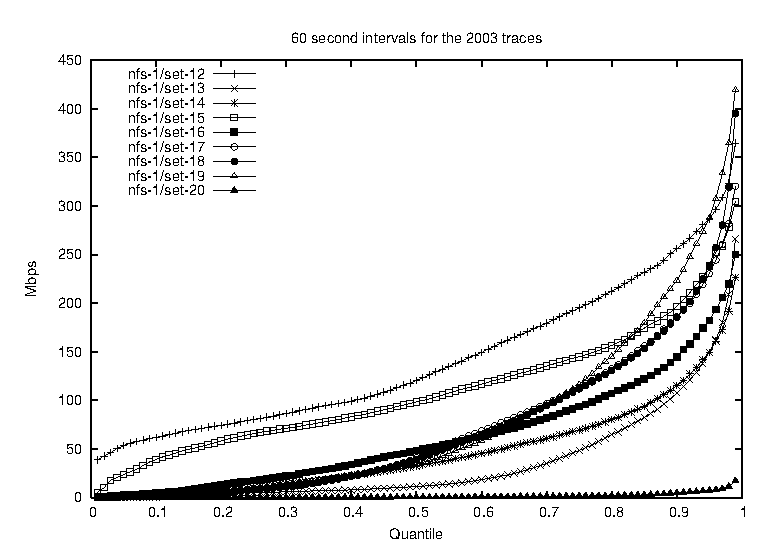
\epsfig{width=2.1in, angle=0, file=graphs/Mbps-nfs-1.ps}
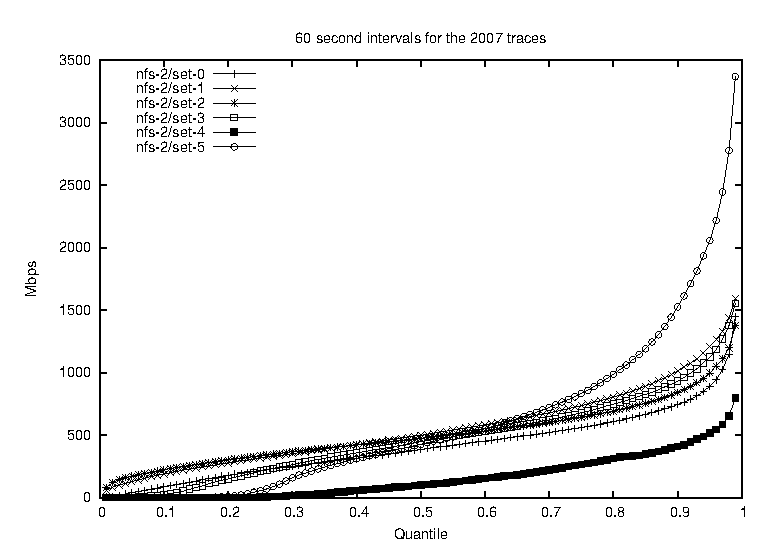
\epsfig{width=2.1in, angle=0, file=graphs/Mbps-nfs-2.ps}
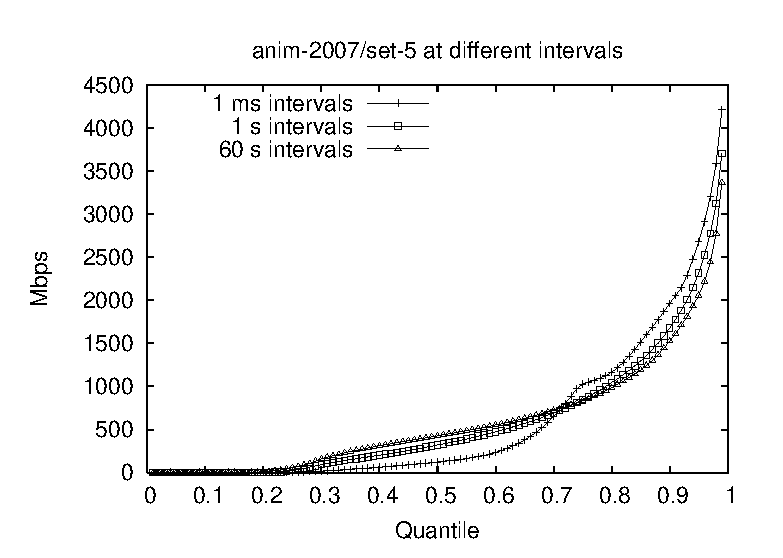
\epsfig{width=2.1in, angle=0, file=graphs/Mbps-nfs-2-set-5.ps}
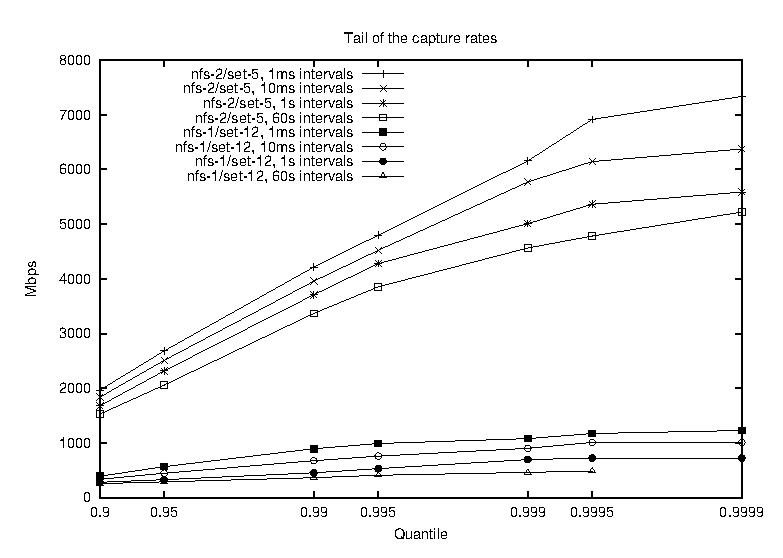
\epsfig{width=2.1in, angle=0, file=graphs/Mbps-tails.ps}
\caption{Bandwidth measured in the collection process.  In figure (c),
animation-2007/set-5 at different intervals is the top group of 4 lines, and
animation-2003/set-12 is the bottom group of 4 lines. animation-2003/set-12 does not go
all the way to the right at 60s intervals because there were
insufficient data points for the 0.9999 quantile.}
\label{fig:bwrolling-mbps}
\end{figure*}

% \begin{figure*}
% 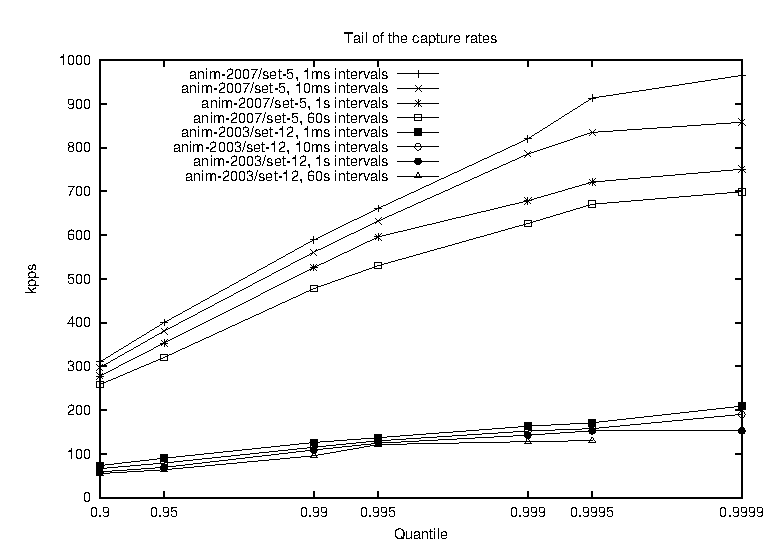
\epsfig{width=2.1in, angle=0, file=graphs/kpps-tails.ps}
% \caption{Tail of the quantiles in Mbps and kpps for the animation-2007 traces.}
% \label{fig:capture-tails}
% \end{figure*}

\subsection{Basic NFS analysis}

% nfs_hostinfo_rates, nfs_hostinfo_rate_quantiles, nfs_hostinfo_cube;
% choose sets nfs-2/set-[2,5]; nfs-1/set-[5,12]
%                     03+10, 06+13 ; 20+42, 27+49

% select from_unixtime(group_time), group_count/3600 where dataset = 'nfs-1/set-12' and group_time is not null and host is null  and operation is null and direction is null and op_dir is null
% nfs-1/set-5: 2003-09-16 .. 2003-09-18
% nfs-1/set-12: 2003-12-09 - 2003-12-10
% nfs-2/set-2: 2007-03-05 .. 2007-03-11
% nfs-2/set-5: 2007-10-12 .. 2007-10-17
% from hostinfo.hg + a few minor tweaks (n/a) for set-5 readdirplus
\begin{table*}
\begin{tabular}{|r||r|r||r|r||r|r||r|r|}
\hline
  & \multicolumn{2}{c||}{animation-2003/set-12} & \multicolumn{2}{c||}{animation-2003/set-5} & \multicolumn{2}{c||}{animation-2007/set-2} & \multicolumn{2}{c|}{animation-2007/set-5} \\
   operation &   Mops & bytes/op &   Mops & bytes/op &   Mops & bytes/op &   Mops & bytes/op \\
%\hline
%     symlink &     0.008 &   201 &     0.000 &    92 &     0.001 &   415 &     0.000 &   458 \\
%       rmdir &     0.204 &   152 &     0.001 &    64 &     0.020 &   167 &     0.002 &   178 \\
%       mkdir &     0.173 &   304 &     0.005 &   193 &     0.071 &   336 &     0.004 &   334 \\
%      rename &     0.028 &   270 &     0.002 &   150 &     0.250 &   367 &     0.055 &   348 \\
%\hline
%      fsinfo &     0.023 &   176 &     0.003 &    72 &     1.352 &   176 &     0.619 &   176 \\
%        link &     0.000 &    86 &     0.000 &    88 &     3.259 &   314 &     0.182 &   322 \\
%        null &     0.259 &     5 &     0.087 &     4 &     1.482 &     4 &     2.808 &     4 \\
%      create &     0.296 &   295 &     0.965 &   200 &     4.639 &   367 &     1.616 &   344 \\
%\hline
%      remove &     0.275 &   136 &     0.641 &    69 &     8.419 &   194 &     1.500 &   186 \\
%     setattr &     0.716 &   133 &     1.075 &   136 &     9.415 &   193 &     6.531 &   192 \\
     readdir &     4.579 &   281 &     1.132 &  3940 &    28.318 &  4089 &    18.350 &  4071 \\
 readdirplus &     0.632 &  2307 &     0.000 &  n/a  &    32.806 &  1890 &    20.271 &  2001 \\
    readlink &     0.081 &    74 &     0.049 &    79 &    25.421 &   204 &    42.335 &   203 \\
      fsstat &    19.875 &    56 &    50.416 &    56 &     0.017 &   180 &     0.003 &   180 \\
       write &    14.546 &  9637 &    30.236 &  7880 &    32.390 & 13562 &    45.177 & 15015 \\
\hline
      lookup &   134.108 &    83 &    82.823 &    92 &   643.854 &   239 &   807.127 &   235 \\
        read &   345.743 &  1231 &   165.969 &  7855 &  1460.669 & 14658 &  1761.199 & 12301 \\
      access &     1.858 &   136 &     0.000 &   136 &  4000.204 &   136 &  3570.404 &   136 \\
     getattr &   244.650 &   104 &   967.961 &   104 &  6598.515 &   124 &  2756.785 &   123 \\
\hline
 {\bf total} &   768.053 &   790 &  1301.364 &  1274 & 12851.102 &  1833 &  9034.968 &  2599 \\
\hline
\end{tabular}

\caption{symlink, rmdir, mkdir, and rename were pruned as there were
fewer than 1 million operations; fsinfo, link, null, create, remove,
and setattr were pruned as there were fewer than 10 million
operations}

\label{table:nfs-stats-overview}
\end{table*}

\begin{figure*}
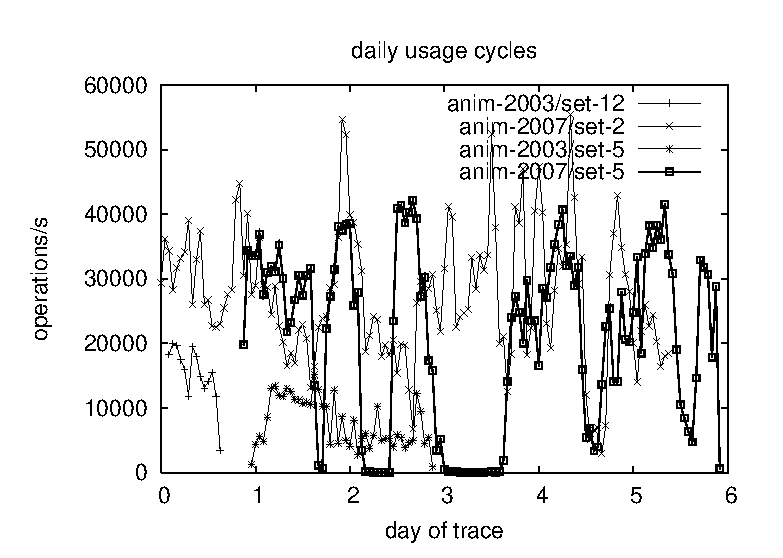
\epsfig{width=2.1in, angle=0, file=graphs/daily-oprate.ps}
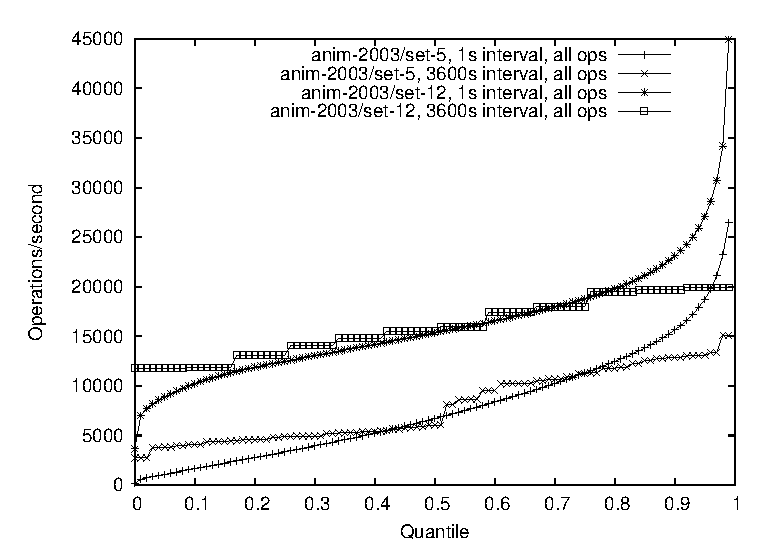
\epsfig{width=2.1in, angle=0, file=graphs/allops-quantile-nfs-1.ps}
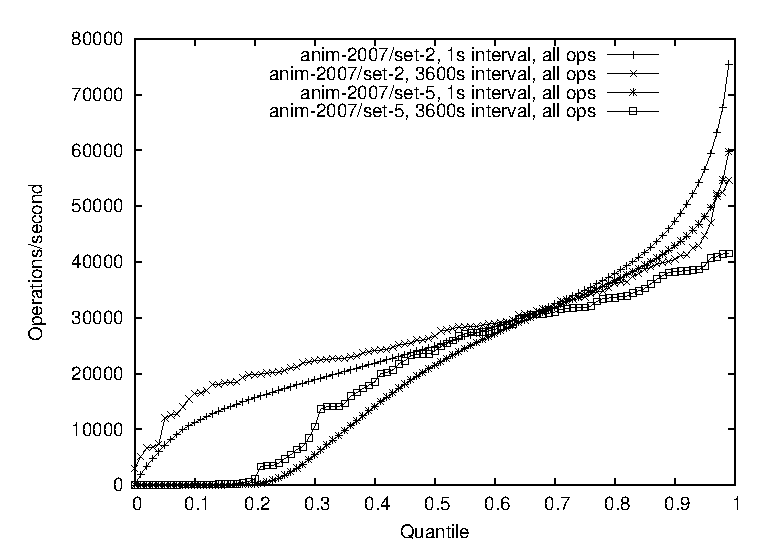
\epsfig{width=2.1in, angle=0, file=graphs/allops-quantile-nfs-2.ps}
\caption{Operation rates, grouped into one hour units (a), and quantiles (b), (c).}
\label{fig:oprates}
\end{figure*}

\begin{figure*}
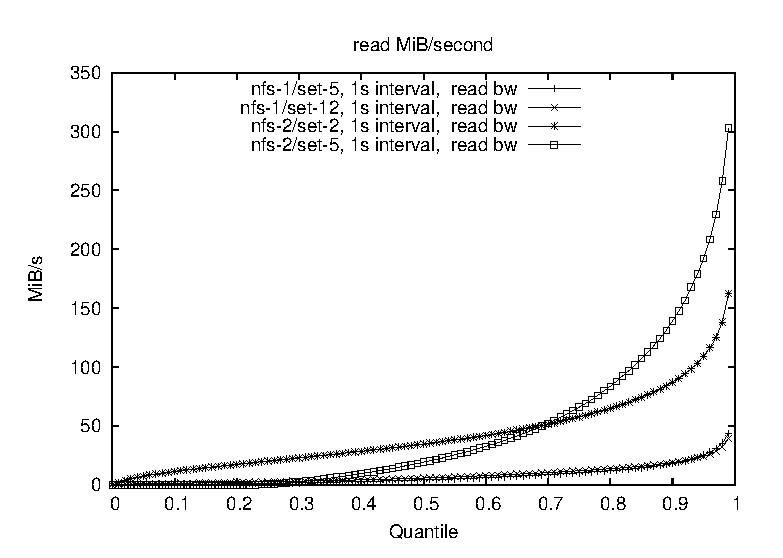
\epsfig{width=2.1in, angle=0, file=graphs/bw-read.ps}
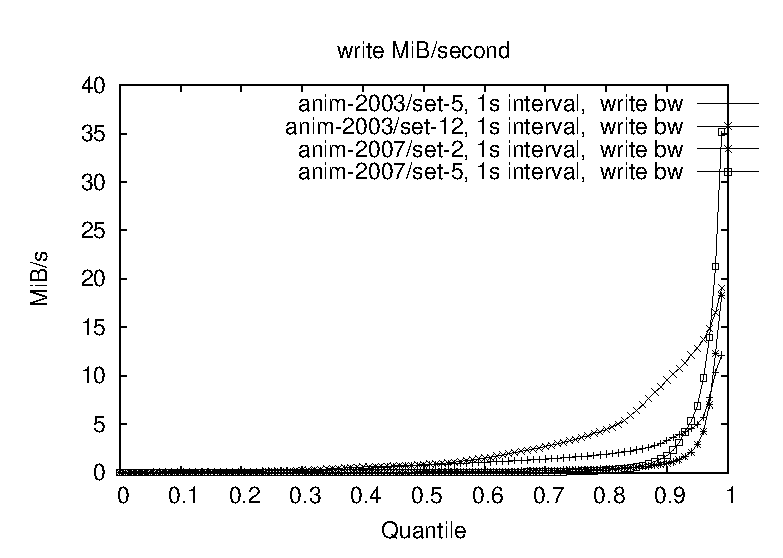
\epsfig{width=2.1in, angle=0, file=graphs/bw-write.ps}
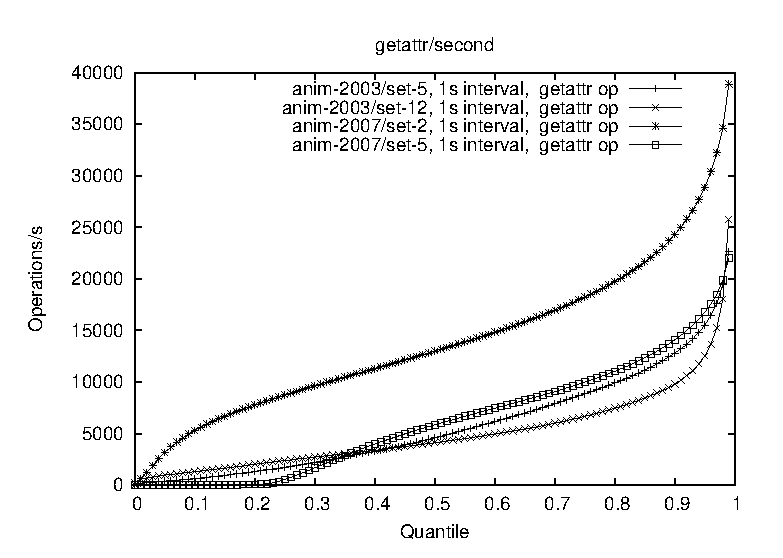
\epsfig{width=2.1in, angle=0, file=graphs/ops-getattr.ps}
\caption{Bandwidth for reads and writes, and operation rate for getattrs in the four traces.}
\label{fig:bw-ops-quantiles}
\end{figure*}

Examining the overall set of operations used by a workload provides
insight into what operations need to be optimized to support the
workload.  Examining the distribution of rates for the workload tells
us if the workload is bursty, and hence we need to handle a higher
rate than would be implied by mean arrival rates, and if there are
periods of idleness that could be exploited.

Table~\ref{table:nfs-stats-overview} provides an overview of all the
operations that occurred in the four traces we are examining in more
detail.  It shows a number of substantial changes in the workload
presented to the NFS subsystem.  First, the read and write sizes have
almost doubled from the animation-2003 to animation-2007 datasets.  This is expected
because the company moved from NFSv2 to NFSv3 between the two
tracing periods, and set the v3 read/write size to 16k.  We asked and
were told they set it to those sized based on some performance
measurements of sequential I/O.  The NFS version switch also accounts
for the increase in access calls (new in v3), and readdirplus (also
new in v3).  

We also see that this workload is incredibly read-heavy.  This is
expected; the animation workload reads a very large amount of
textures, models, etc. to produce a relatively small output frame.
However, we believe that our traces under-estimate the number of write
operations.  We discuss the write operation underestimation below.
The abnormally low read size for set-12 occurred because
that filer was handling a large number of stale FH requests.  The
replies were therefore small and pulled down the bytes/operation.  We
see a lot more getattr operations in set-5 than set-12 because set-12
is a filer behind some nfs-caches, whereas set-5 is the workload
before the nfs-caches.

Table~\ref{table:99quant-differences} and
figure~\ref{fig:oprates}(b,c) shows how long averaging intervals
can distort the load placed on the storage system.  If we were to
develop a storage system for the hourly loads reported in most papers,
we would fail to support the substantially higher near peak (99\%)
loads seen in the data.  It also hides periods of idleness
that could be used for incremental scrubbing and data reorganization.

We include figure~\ref{fig:oprates}(a) because it is the traditional
graph that shows daily cycles.  We do not have quite as strong daily
cycles because animation companies are good at keeping their compute
clusters busy overnight, but we can see for animation-2007/set-5 the effect of
the weekends where the load on the system drops nearly to 0.

Figure~\ref{fig:bw-ops-quantiles} shows the read and write MiB/s and the
getattr operations/s.  It shows that relative to the amount of data
being transferred, the number of getattrs has been reduced, likely a
result of the transition from NFSv2 to NFSv3.  The graph shows the
payload data transferred, so it includes the offset and filehandle of
the read request, and the size and data in the reply, but does not
include IP headers or NFS RPC headers.  It shows that the NFS system
is driven heavily, but not excessively, and it seems to imply that the
write bandwidth has gotten more bursty, but has stayed roughly
constant.  

This result led us to further analyze the data.  We were surprised
that that write bandwidth would not increase, even though it is not
implausible as the frame output size has not increased.  We analyzed
the traces to look for missing operations in the sequence of
transaction ids, automatically inferring if the client is using a
big-endian or little-endian counter.  The initial results looked quite
good, animation-2007/set-2 showed 99.7\% of the operations were in sequence,
animation-2007/set-5 showed 98.4\%, and counting the skips of 128 transactions
or less, we found only 0.21\% and 0.50\% respectively (the remaining
entries were duplicates or ones that we could not positively tell if
they were in sequence or a skip).  However, when we looked one level
deeper at the operation that preceded a skip in the sequence, we found
that 95\% of the skips followed a write operation for set-2, and 45\%
for set-5.  The skips in set-2 could increase the write workload by a
factor of 1.5x if all missing skips after writes are associated with
writes.  We expected a fair number of skips for set-5 since we
experienced packet loss under load, but we did not expect it for
set-2.

Further examination indicated that the problem came about because we
followed the same parsing technique for TCP packets as was used in
nfsdump2~\cite{ellardTraces}.  We started at the beginning of the
packet and parsed all of the RPCs that we found that matched all
required bits to be RPCs.  Unfortunately, over TCP, two back to back
writes will not align the second write RPC with the packet header, and
we will miss subsequent operations until they re-align with the packet
start.  While the fraction of missing operations is small, they are
biased toward writes (read replies can only be affected if the second
read reply is close enough to the first that they are combined).  This
leads us to one of our lessons, extensive validation of the conversion
tool is important.  Both validation through validation statistics, and
through the use of a known workload that exercises the capture tools.
An NFS replay tool~\cite{NingningFast05} could be used to validate
that the captured workload is the one that was replayed.  This
comparison has been done to validate a block based replay
tool~\cite{AndersonFast04}, but has not been done to validate a
capture tool, as that work simply assumed capture was correct.  We
expect to partially ameliorate this problem before the final paper
because we have the complete packet traces, including any packets that
we could not parse.  We can therefore use the timing information from
requests and replies to identify gaps in the dataset and determine how
many bytes were skipped.  This will allow us to approximate the number
of missing writes.  Preservation of lower level information is a
lesson we got right, and it will allow us to partially reconstruct
flaws in the traces.  We believe a similar flaw is present in earlier
traces~\cite{ellardTraces} because the same parsing technique was
used, we do not know how much those traces were affected.

% select dataset, group_seconds, operations_per_second from xnfs_hostinfo_rate_quantiles where host is null and direction = 'send' and operation is null and op_dir is null and quantile = 0.99
\begin{table}
\begin{tabular}{|r|r|r|r|}
\hline
dataset & 1s ops/s & 3600s ops/s & ratio \\
\hline
animation-2003/set-5  & 26445  & 15110 & 1.75x \\
animation-2003/set-12 & 44926 & 19923 & 2.25x \\
animation-2007/set-2  & 75457 & 54657 & 1.38x \\
animation-2007/set-5  & 59726.5 & 41550 & 1.44x \\
\hline
\end{tabular}
\caption{Ratio between operation rates at 1 second and one hour grouping sizes}
\label{table:99quant-differences}
\end{table}

\subsection{File sizes}

\begin{figure}
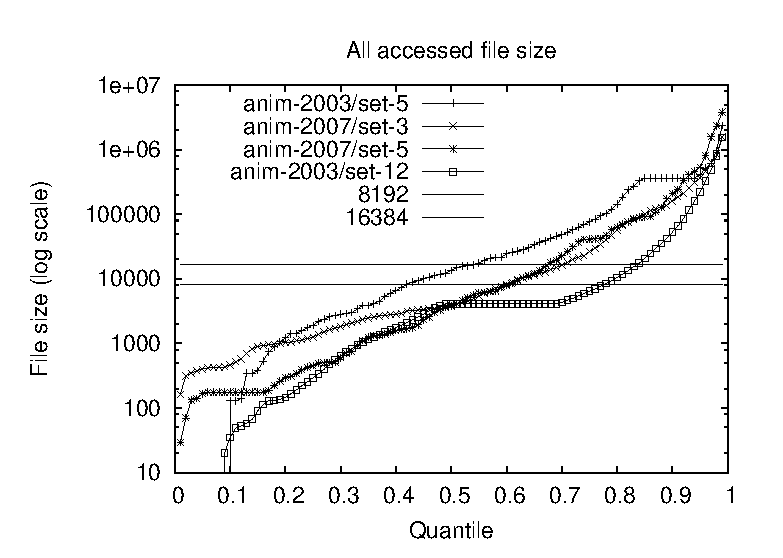
\epsfig{width=2.1in, angle=0, file=graphs/file-size.ps}
\caption{File size distribution for all accessed files.}
\label{fig:file-size}
\end{figure}

File sizes affect the potential internal fragmentation for a
filesystem.  They affect the maximum size of I/Os that could be
executed, and they affect the potential sequentiality in a workload.

Figure~\ref{fig:file-size} shows the size of files accessed in our
traces.  It shows that the files in the animation workload are in
general very small, as 40-80\% of the files are smaller than 8k, and
hence will be read in a single I/O for the 2003 traces.  70\% of the
files are smaller than 16k for the 2007 traces, and hence will be read
in a single I/O.  While there are larger files in the traces, 99\% of
the files are smaller than 10MB.  The small file sizes present in this
workload, and the preponderance of writes suggest that a flash file
system~\cite{Kawaguchi95aflash-memory} or MEMS file
system~\cite{SchlosserFast04} could support a substantial portion of
the workload.

\subsection{Sequentiality}

\begin{figure*}
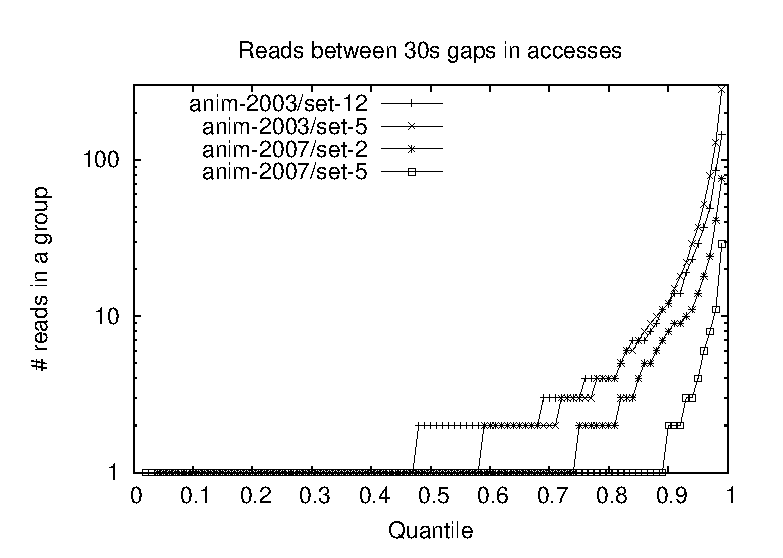
\epsfig{width=2.1in, angle=0, file=graphs/seq-read-group-counts.ps}
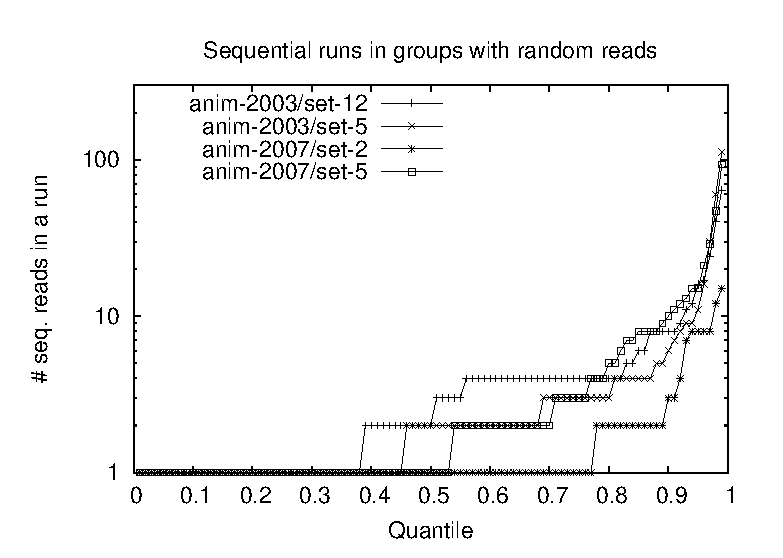
\epsfig{width=2.1in, angle=0, file=graphs/seq-in-random-seq-count.ps}
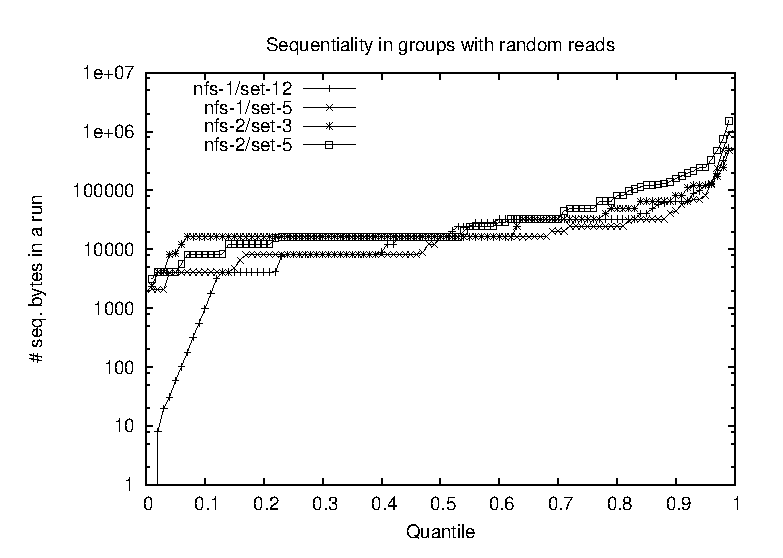
\epsfig{width=2.1in, angle=0, file=graphs/seq-in-random-seq-bytes.ps}
\caption{number of reads in a single group (more than 30s gap between I/Os); }
\label{fig:seq-analysis}
\end{figure*}

\begin{figure}
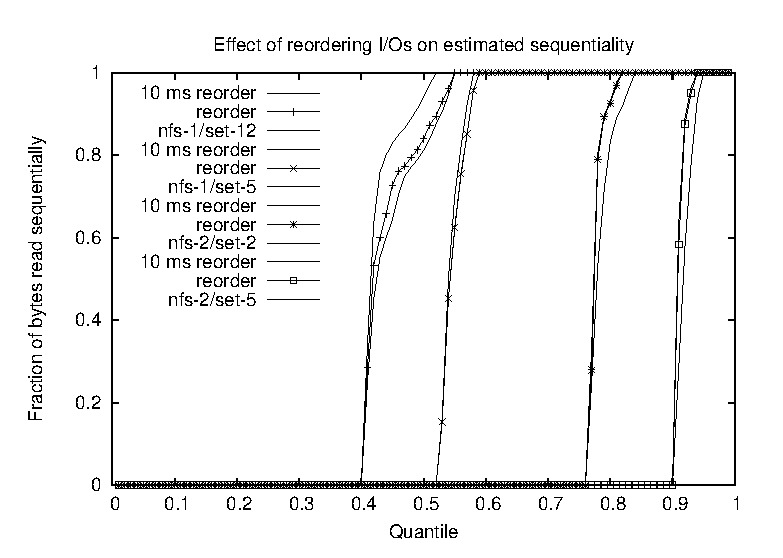
\epsfig{width=2.1in, angle=0, file=graphs/seq-bytes-compare.ps}
\caption{Negligible effect of reordering I/Os to improve estimated sequentiality.}
\label{fig:seq-bytes-compare}
\end{figure}

Sequentiality is one of the most important properties for storage
systems because disks are much more efficient when handling sequential
data rather than random accesses.  Prior work has presented
various methods for calculating sequentiality.  Both
Ellard~\cite{EllardFast03} and Leung~\cite{LeungUsenix08} split accesses
into groups and calculate the sequentiality within the group.  Ellard
emulates opens and closes by looking for 30s groups in the access
pattern.  Ellard tolerates small gaps in the request stream as
sequential, e.g. an I/O of 7k at offset 0 followed by an I/O of 8k at
offset 8k would be considered sequential.  Ellard also re-orders I/Os
to deal with client-side reordering. In particular Ellard looks
forward a constant amount from the request time to find I/Os that
could make the access pattern more sequential.  This constant was
determined empirically.  Leung treats the first I/O after an open as
sequential.

We prefer to only reorder within overlapping requests. Given two I/Os,
A, and B, if the request-reply intervals overlap, then we are willing
to re-order the requests to improve estimated sequentiality.  We
believe this is a better model because the NFS server could have a
change to re-order those I/Os.  In practice
figure~\ref{fig:seq-bytes-compare} shows that for our traces this
reordering makes little difference.  Allowing reordering an additional
10ms beyond the reply of I/O A slightly increases the sequentiality,
but generally not much more than just for overlapping requests.

We also decide on whether the first I/O is sequential or random based
on additional I/Os.  If the second I/O (after any reordering) is
sequential to the first one, than the first I/O is sequential,
otherwise it is random.  If there is only one I/O to a particular
file, then we consider the I/O to be random since the NFS server would
have to reposition to that file to start the read.  

Given our small file sizes, it turns out that most accesses count as
random because they read the entire file in a single I/O.  We can see
this in figure~\ref{fig:seq-analysis}(a) which shows the number of
reads in a group.  Most groups are single I/O groups (70-90\% in the
2007 traces).  We see about twice as many I/Os in the 2003 traces,
because the I/Os in the 2003 traces are only 8KiB rather than 16KiB.

Sequential runs within a random group turns out to be more
interesting.  Figure~\ref{fig:seq-analysis}(b,c) show the number of
I/Os and the number of bytes accessed in sequential runs within a
random group.  We can see that if we start accessing a file at random,
most (50-80\%) of the time we will do single or double I/O accesses.
However we can also see that we can get some extended runs within a
random group, although 99\% of the runs are less than 1MB.

% select dataset,operation, max(mean_operations_per_second) from xnfs_hostinfo_rates where group_seconds = 1 and host is null and direction = 'send' and operation is not null and op_dir is null and mean_operations_per_second > 300 group by dataset,operation order by operation
% --> access, fsstat, getattr, lookup, read, write 

\fix{5. Cram another analysis in here: file size distribution by
unique and access, or stack-distance}


\section{Conclusions}
\label{sec:conclusion}

We have described three improved techniques for packet capture on
networks.  The easily adopted technique should allow anyone capturing
NFS, CIFS, or iSCSI traffic from moderate performance storage systems
($\leq$1Gbit) to capture traffic with no losses.  The most advanced
technique allows lossless capture for 5-10Gbit storage systems, which
is at the high end of most file storage systems. The primary lesson
from this part of the work is that lossless 1Gbit packet capture is
straightforward and up to 10Gbit is possible with an investment in
development time or specialized hardware.

We have provided guidelines for conversion for future practitioners:
parallelizing the conversion, retaining lower-level information, using
reversible anonymization, approaches for testing the conversion tools,
and tagging the trace data with version information.

We have described our binary storage format, which uses chunked
compression with multiple possible compression techniques, typed
relational-style data structuring, delta encoding, and type-safe,
high-speed accessors.  It improves over prior storage formats by up to
100$\times$.

We have described our techniques for improved memory and perforance
efficiency to enable analysis of very large data sets.  We 
explained the cube and approximate quantile techniques that we adopted
from the database literature, and our hashtable, rotating hash-map, and
plotting techniques that we use for analyzing the data.

We have analyzed our NFS workload examining some of the different
properties found in a feature animation workload and demonstrating
that our techniques are effective.  We found that our workload had
much more activity than previously described workloads, and that the
file size and sequentality is different than those workloads.

Finally, to allow future practitioners to collect traces more easily,
and use our traces for analysis and simulation, we have open sourced
them at {\tt http://tesla.hpl.hp.com/opensource}.

\section{Acknowledgements}

The author would like to thank Alistair Veitch, Jay Wylie, Kimberly
Keeton, our shepherd Daniel Ellard and the anonymous reviewers for
their comments that have improved our paper.

{
\bibliography{references}
\bibliographystyle{plain}
}


\end{document}







